\documentclass[tikz,border=8pt]{standalone}

\usepackage{amsmath}
\usetikzlibrary{arrows.meta,positioning}

\definecolor{agentblue}{HTML}{2F6F9F}
\definecolor{actionred}{HTML}{D96C5F}
\definecolor{systemgreen}{HTML}{4F9D8A}
\definecolor{softgray}{HTML}{6B7280}

\begin{document}
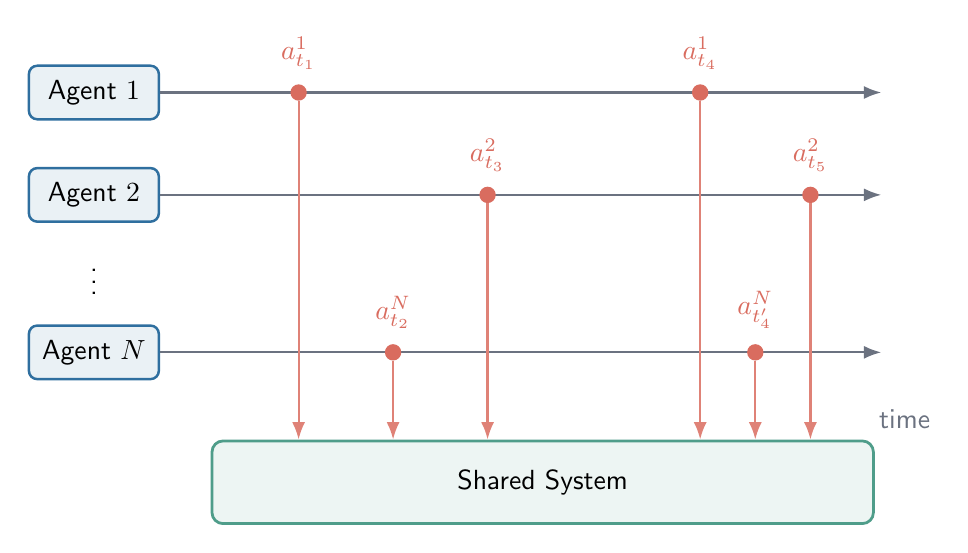
\begin{tikzpicture}[
    font=\sffamily,
    >=Latex,
    agent/.style={
        draw=agentblue,
        fill=agentblue!10,
        rounded corners=3pt,
        minimum width=1.65cm,
        minimum height=0.68cm,
        line width=0.9pt
    },
    event/.style={
        circle,
        draw=actionred,
        fill=actionred,
        minimum size=5.5pt,
        inner sep=0pt
    },
    system/.style={
        draw=systemgreen,
        fill=systemgreen!10,
        rounded corners=4pt,
        minimum width=8.4cm,
        minimum height=1.05cm,
        line width=1pt
    }
]

% Agents
\node[agent] (a1) at (0,4.5) {Agent $1$};
\node[agent] (a2) at (0,3.2) {Agent $2$};
\node at (0,2.2) {$\vdots$};
\node[agent] (an) at (0,1.2) {Agent $N$};

% Independent timelines
\foreach \node/\y in {a1/4.5,a2/3.2,an/1.2} {
    \draw[-{Latex[length=2.2mm]},softgray,line width=0.75pt]
        (\node.east) -- (10.0,\y);
}

% Asynchronous action events
\node[event] (e11) at (2.6,4.5) {};
\node[above=2pt of e11, text=actionred] {$a^1_{t_1}$};
\node[event] (e12) at (7.7,4.5) {};
\node[above=2pt of e12, text=actionred] {$a^1_{t_4}$};

\node[event] (e21) at (5.0,3.2) {};
\node[above=2pt of e21, text=actionred] {$a^2_{t_3}$};
\node[event] (e22) at (9.1,3.2) {};
\node[above=2pt of e22, text=actionred] {$a^2_{t_5}$};

\node[event] (en1) at (3.8,1.2) {};
\node[above=2pt of en1, text=actionred] {$a^N_{t_2}$};
\node[event] (en2) at (8.4,1.2) {};
\node[above=2pt of en2, text=actionred] {$a^N_{t_4'}$};

% Shared system
\node[system] (sys) at (5.7,-0.45) {Shared System};

% Actions reach the same system at different times
\foreach \event in {e11,e12,e21,e22,en1,en2} {
    \draw[-{Latex[length=2.2mm]},actionred!85,line width=0.8pt]
        (\event.south) -- (\event.south |- sys.north);
}

\node[text=softgray,anchor=west] at (9.85,0.35) {time};

\end{tikzpicture}
\end{document}
